\chapter{فرمنت‌ها، نرم‌افزار \eng{Praat} و فضای واکه‌ای}

در جلسهٔ پیش، سیگنال گفتار را به مؤلفه‌های فرکانسی تجزیه کردیم و با هارمونیک‌ها، اسپکتروگرام و مدل منبع–فیلتر آشنا شدیم. هدف این جلسه گام بعدی است: چگونه از روی سیگنال صوتی، ویژگی‌های \term{آکوستیکی}{Acoustic} مانند \eng{F1} و \eng{F2} را اندازه بگیریم و آن‌ها را به ویژگی‌های \term{تولیدی}{Articulatory} مانند ارتفاع و جلو یا عقب‌بودن زبان نگاشت کنیم. ابزار عملی این کار نرم‌افزار \eng{Praat} است و نتیجهٔ کار، \term{فضای واکه‌ای}{Vowel Space} است که در گفتاردرمانی، تشخیص صدای جعلی و پایش بیماری‌های عصبی به کار می‌رود.

\begin{figure}[htbp]
\centering
\begin{tikzpicture}[rtl, 
  node distance=0.45cm,
  stage/.style={draw, rounded corners=3pt, fill=blue!6, text width=2.6cm, align=center, minimum height=1.25cm, font=\small},
  arr/.style={-{Stealth[length=2mm]}, thick}
]
\node[stage] (a) {ضبط یا بازکردن صوت};
\node[stage, left=of a] (b) {تحلیل: طیف‌نگاره، \lr{Pitch}، \lr{Formant}};
\node[stage, left=of b] (c) {برچسب‌گذاری با \lr{TextGrid}};
\node[stage, below=1.1cm of a] (d) {اندازه‌گیری \lr{F1} و \lr{F2} هر واکه};
\node[stage, left=of d] (e) {ساخت نمودار فضای واکه‌ای};
\node[stage, left=of e] (f) {مقایسه و کاربرد: درمان، جعل، پایش};
\draw[arr] (a) -- (b);
\draw[arr] (b) -- (c);
\draw[arr] (c.south) -- ++(0,-0.55) -| (d.north);
\draw[arr] (d) -- (e);
\draw[arr] (e) -- (f);
\end{tikzpicture}
\caption{زنجیرهٔ مفهومی جلسه: از ضبط صوت تا کاربردهای فضای واکه‌ای (شکل افزوده).}
\end{figure}

\section{مرور کوتاه: از فرکانس پایه تا فرمنت}
جزئیات فوریه، هارمونیک‌ها، اسپکتروگرام و مدل منبع–فیلتر در فصل ۳ آمده است. این‌جا فقط نکته‌هایی را که در ابتدای این جلسه برای پاسخ به پرسش‌ها مرور شد، فشرده می‌آوریم.

\begin{itemize}
  \item \textbf{فرکانس پایه.} اگر یک موج تناوبی در هر $T$ ثانیه یک دورهٔ کامل بزند، $f_0=1/T$ است. برای تشخیص زیروبمی (\eng{Pitch}) به جای همهٔ نوسان‌های ریز، تکرار قله‌های اصلی، یعنی کندترین الگوی تناوبی، را در نظر می‌گیریم. در مدل منبع–فیلتر، $f_0$ به \emph{منبع} (چین‌های صوتی) و فرمنت‌ها به \emph{فیلتر} (مجرای صوتی) مربوط‌اند.
  \item \textbf{ضریب فوریه.} خروجی تبدیل فوریه برای هر مؤلفهٔ فرکانسی یک عدد مختلط $X=a+jb$ است. اندازهٔ آن $|X|=\sqrt{a^2+b^2}$ میزان مشارکت آن فرکانس در سیگنال (\eng{Magnitude}) و زاویهٔ آن فاز است.
  \item \textbf{دامنه و \eng{Magnitude}.} دامنه (\eng{Amplitude}) مقدار سیگنال در حوزهٔ زمان است؛ در اسپکتروگرام محور افقی زمان، محور عمودی فرکانس و رنگ، \eng{Magnitude} (یا توان) هر مؤلفه است. این دو را نباید یکی دانست، هرچند به هم مرتبط‌اند. رنگ گرم‌تر یعنی مقدار طیفی بیشتر.
  \item \textbf{تعامد.} موج‌های مبنا باید نسبت به هم متعامد باشند تا هر کدام مؤلفه‌ای مستقل را بسنجند: ضرب داخلی دو موج در بازه صفر باشد، یعنی $\int_0^T x_1(t)x_2(t)\,dt=0$ یا در حالت گسسته $\sum_{n=0}^{N-1}x_1[n]x_2[n]=0$. موج‌هایی که در بازهٔ $T$ تعداد صحیحی دوره می‌زنند (فرکانس‌های $1/T,\,2/T,\,3/T,\dots$) چنین مجموعه‌ای می‌سازند.
  \item \textbf{هارمونیک‌ها.} فرکانس‌های هارمونیک $f_n=nf_0$ هستند، اما ضریب برخی از آن‌ها می‌تواند صفر یا ناچیز باشد. مثال کلاس موج مربعی با چرخهٔ کاری ۵۰ درصد بود که فقط هارمونیک‌های فرد ($f_0,3f_0,5f_0,\dots$) را دارد؛ نبودن هارمونیک زوج یعنی ضریبش صفر است، نه این‌که از مجموعهٔ فرکانس‌های مبنا بیرون باشد.
\end{itemize}

\begin{exambox}{پرسش و پاسخ: آیا تعداد هارمونیک‌ها بی‌نهایت است؟}
از نظر ریاضی مضرب‌های صحیح $f_0$ بی‌پایان‌اند، اما در عمل بالاترین فرکانس قابل تحلیل را نرخ نمونه‌برداری (حداکثر نصف آن، قضیهٔ نایکویست) و هدف تحلیل محدود می‌کند. در تحلیل گفتار فقط بخشی از طیف که برای مسئله اطلاعات مفید دارد بررسی می‌شود. برای تعیین «هارمونیک‌های مهم» می‌توان بر اندازهٔ ضرایب آستانه گذاشت.
\end{exambox}

\subsection{هارمونیک در برابر فرمنت}
هارمونیک‌ها ویژگی \emph{سیگنال تناوبی} (منبع) هستند، در حالی که \term{فرمنت‌ها}{Formants} نواحی تشدید \emph{مجرای صوتی} (فیلتر) را توصیف می‌کنند و به صورت برآمدگی‌های پوش طیفی دیده می‌شوند. با نگاه به هارمونیک‌ها تنها نمی‌توان فهمید زبان در کجاست؛ برای تحلیل نحوهٔ تولید واکه باید فرمنت‌ها را استخراج کرد. یکی از روش‌های رایج تخمین فرمنت، \term{کدگذاری پیش‌بینی خطی}{Linear Predictive Coding (LPC)} است؛ روش‌های دیگری هم وجود دارند که از محدودهٔ این بخش بیرون‌اند.

\begin{table}[htbp]
\centering
\caption{مقایسهٔ اسپکتروگرام پهن‌باند و باریک‌باند}
\begin{tabular}{p{3.2cm}p{5.2cm}p{5.2cm}}
\toprule
ویژگی & \eng{Wideband} & \eng{Narrowband} \\
\midrule
طول پنجرهٔ تحلیل & کوتاه‌تر (حدود ۵ میلی‌ثانیه) & بلندتر \\
تفکیک زمانی & بیشتر & کمتر \\
تفکیک فرکانسی & کمتر & بیشتر \\
ظاهر طیف & نواحی پهن انرژی؛ فرمنت‌ها و تغییرات سریع دیده می‌شوند & خطوط هارمونیکی جداگانه \\
کاربرد & دنبال‌کردن فرمنت‌ها و حرکت اندام‌ها & بررسی هارمونیک‌ها و $f_0$ \\
\bottomrule
\end{tabular}
\end{table}

وضوح زمانی مهم است چون زبان و سایر اندام‌های گفتار سریع جابه‌جا می‌شوند و برای نگاشت آکوستیک به تولید باید این تغییرات را دنبال کرد. به همین دلیل برای مشاهدهٔ فرمنت‌ها از نمای پهن‌باند استفاده می‌کنیم.

\section{نگاشت ویژگی‌های آکوستیکی به ویژگی‌های تولیدی}
در آواشناسی تولیدی (فصل ۲) واکه‌ها را با موقعیت زبان توصیف می‌کنیم: بالا یا پایین (بسته یا باز)، جلو یا عقب، و گرد یا غیرگرد بودن لب‌ها. در پردازش گفتار معمولاً موقعیت واقعی زبان را مستقیم اندازه نمی‌گیریم؛ در عوض ویژگی‌های آکوستیکی را از صوت استخراج و برای توصیف فضای واکه‌ای استفاده می‌کنیم. دو فرمنت اول بیشترین نقش را دارند.

\begin{definitionbox}{نگاشت \eng{F1} و \eng{F2} به ویژگی‌های تولیدی}
\begin{itemize}
  \item \term{فرمنت اول}{F1}: رابطهٔ \emph{معکوس} با ارتفاع زبان. زبان بالاتر (واکهٔ بسته) $\Leftarrow$ \eng{F1} کمتر؛ زبان پایین‌تر (واکهٔ باز) $\Leftarrow$ \eng{F1} بیشتر.
  \item \term{فرمنت دوم}{F2}: مرتبط با جلو یا عقب بودن زبان. زبان جلوتر $\Leftarrow$ \eng{F2} بیشتر؛ زبان عقب‌تر $\Leftarrow$ \eng{F2} کمتر.
  \item \term{گرد شدن لب}{Lip Rounding}: باعث افت \eng{F2} می‌شود.
\end{itemize}
\end{definitionbox}

\begin{table}[htbp]
\centering
\caption{رابطهٔ جایگاه واکه با \eng{F1} و \eng{F2}}
\begin{tabular}{lcc}
\toprule
جایگاه واکه & \eng{F1} & \eng{F2} \\
\midrule
زبان بالا (بسته) & کم & بسته به جلو یا عقب‌بودن \\
زبان پایین (باز) & زیاد & بسته به جلو یا عقب‌بودن \\
زبان جلو & بسته به ارتفاع & زیاد \\
زبان عقب (و/یا لب گرد) & بسته به ارتفاع & کم \\
\bottomrule
\end{tabular}
\end{table}

در جلسهٔ ۳ با دو مثال شهودی هم آشنا شدیم: جلو آوردن زبان محفظهٔ جلوی دهان را کوچک می‌کند و \eng{F2} بالا می‌رود، و طول مجرای صوتی روی دامنهٔ فرمنت‌ها اثر دارد (مجرای بلندتر، فرمنت‌های پایین‌تر).

\begin{correctionbox}{دقت در رابطهٔ «ارتفاع زبان = \eng{F1}»}
قواعد فوق تقریبی هستند، نه قانونی دقیق. فرمنت‌ها تشدیدهای کل مجرای صوتی‌اند و به شکل مجموع سطح مقطع مجرا، از چین‌های صوتی تا لب‌ها، بستگی دارند، نه یک «حفرهٔ» مشخص. \eng{F1} علاوه بر ارتفاع زبان به باز بودن فک و تنگی حلق نیز حساس است (واکهٔ باز: دهان باز و حلق تنگ‌تر، \eng{F1} بالا). \eng{F2} به جلو یا عقب بودن زبان و گردی لب‌ها وابسته است. به همین دلیل واکهٔ عقبی گرد مانند \eng{/u/} هم \eng{F1} هم \eng{F2} پایین دارد. پرسش دانشجویی «آیا این رابطه قانون ثابت است؟» با همین نگاه پاسخ داده شد: رابطهٔ \eng{F1} با ارتفاع و \eng{F2} با جلوآمدگی یک قاعدهٔ کلی آواشناختی است، نه رابطه‌ای بدون استثنا برای همهٔ واکه‌ها و همهٔ افراد. هنگام بررسی یک گروه جدید این رابطه را از پیش «تعریف» نمی‌کنیم؛ مقادیر واقعی را اندازه می‌گیریم و تفاوت‌ها را تفسیر می‌کنیم.
\end{correctionbox}

\begin{addedbox}{مثال عددی: لولهٔ یکنواخت و اثر طول مجرا}
مجرای صوتی در حالت خنثی را می‌توان با لولهٔ یک‌سر بسته (چین‌های صوتی) و یک‌سر باز (لب‌ها) مدل کرد. فرمنت‌ها در این مدل برابرند با
\[
F_n=\frac{(2n-1)\,c}{4L},\qquad n=1,2,3,\dots
\]
که $c\approx 35000$ سانتی‌متر بر ثانیه سرعت صوت در هوای گرم و مرطوب مجرا و $L$ طول مجرا است. برای مرد بزرگسال با $L\approx 17{,}5$ سانتی‌متر:
\[
F_1=\frac{35000}{4\times17.5}=500\ \text{Hz},\quad F_2=1500\ \text{Hz},\quad F_3=2500\ \text{Hz}.
\]
برای مجرایی کوتاه‌تر با $L=11$ سانتی‌متر (مثلاً کودک): $F_1\approx 795$ و $F_2\approx 2386$ هرتز. این همان دلیلی است که مقادیر فرمنت زنان و کودکان بالاتر از مردان است و فضای واکه‌ای باید برای هر گروه جداگانه ساخته شود. این مدل فقط تقریب مرتبهٔ اول است و اثر شکل زبان را در نظر نمی‌گیرد.
\end{addedbox}

\section{کار عملی با \eng{Praat}}
\eng{Praat} نرم‌افزار رایگان و متن‌باز تحلیل و برچسب‌گذاری گفتار است که توسط \eng{Paul Boersma} و \eng{David Weenink} در دانشگاه آمستردام توسعه یافته است. استاد آن را برای پل زدن میان ویژگی‌های آکوستیکی و تولیدی معرفی کرد. در این جلسه تمرکز بر دو کار بود: استخراج فرمنت‌ها و برچسب‌گذاری (\eng{Annotation}).

\subsection{ضبط یا بازکردن صوت و محیط تحلیل}
استاد چند واکه («ای»، «آ»، «او») را ضبط کرد و با نام \eng{Test} ذخیره کرد. در محیط تحلیل \eng{Praat} سه لایه روی هم دیده می‌شود:
\begin{itemize}
  \item \textbf{شکل موج} در بالا.
  \item \term{طیف‌نگاره}{Spectrogram} در پس‌زمینه.
  \item منحنی آبی‌رنگ \eng{Pitch} (فرکانس پایه) و نقطه‌ها یا خطوط قرمز \eng{Formants} که روی طیف‌نگاره رسم می‌شوند.
\end{itemize}
با کلیک روی هر لحظه از سیگنال، مقدار فرمنت‌ها در همان لحظه نمایش داده می‌شود. نمونهٔ نمایش‌داده‌شده در کلاس در یک لحظه چنین بود: \eng{F1} حدود ۳۴۰ هرتز، \eng{F2} حدود ۲۰۰۰ هرتز، \eng{F3} حدود ۳۰۰۰ هرتز و \eng{F4} نیز قابل نمایش است. این اعداد فقط یک اندازه‌گیری لحظه‌ای هستند (الگوی آن شبیه واکهٔ بسته و جلویی \eng{/i/} است) و برای همهٔ واکه‌ها ثابت نیستند. واحد فرمنت‌ها هرتز است.

\begin{addedbox}{راهنمای گام‌به‌گام \eng{Praat}}
\begin{enumerate}
  \item \textbf{ضبط:} در پنجرهٔ اشیا (\eng{Objects}) از منوی \lr{New $\rightarrow$ Record mono Sound...} استفاده کنید؛ پس از ضبط \lr{Save to list} را بزنید. فایل موجود را با \lr{Open $\rightarrow$ Read from file...} بخوانید. برای ضبط با کیفیت، میکروفون نزدیک و محیط ساکت و نرخ نمونه‌برداری ۴۴۱۰۰ یا ۱۶۰۰۰ هرتز مناسب است.
  \item \textbf{نمایش:} شیء \lr{Sound} را انتخاب و دکمهٔ \lr{View \& Edit} را بزنید.
  \item \textbf{لایه‌های تحلیل} در منوهای ویرایشگر: \lr{Spectrum $\rightarrow$ Show spectrogram}، \lr{Pitch $\rightarrow$ Show pitch}، \lr{Intensity $\rightarrow$ Show intensity}، \lr{Formant $\rightarrow$ Show formants}. هر منو یک گزینهٔ \lr{... settings} برای تنظیم پارامترها دارد.
  \item \textbf{پرسش مقدار:} نشانگر را روی نقطه‌ای بگذارید یا یک بازه را انتخاب کنید و از \lr{Formant $\rightarrow$ Get first formant} یا \lr{Get second formant} و مشابه آن‌ها (برای \eng{Pitch} و \eng{Intensity} هم گزینهٔ \lr{Get} وجود دارد) استفاده کنید. برای بازهٔ انتخاب‌شده معمولاً میانگین گزارش می‌شود.
\end{enumerate}
\end{addedbox}

\subsubsection{تنظیمات مهم}
\begin{addedbox}{مقادیر پیش‌فرض و تنظیم‌های پیشنهادی \eng{Praat}}
مقادیر زیر پیش‌فرض‌های متداول ویرایشگر \eng{Praat} هستند (ممکن است در نسخه‌های مختلف اندکی تفاوت داشته باشند).
\begin{itemize}
  \item \textbf{طیف‌نگاره:} بازهٔ نمایش (\eng{View range}) ۰ تا ۵۰۰۰ هرتز؛ طول پنجره (\eng{Window length}) $0.005$ ثانیه، یعنی پهن‌باند؛ بازهٔ پویا (\eng{Dynamic range}) ۷۰ دسی‌بل. افزایش طول پنجره (مثلاً $0.03$ ثانیه) نمای باریک‌باند می‌دهد.
  \item \textbf{\eng{Pitch}:} کف جست‌وجو حدود ۷۵ هرتز و سقف حدود ۵۰۰ تا ۶۰۰ هرتز. توصیهٔ مرسوم: مردان ۷۵ تا ۳۰۰ و زنان ۱۰۰ تا ۵۰۰ هرتز. بازهٔ نادرست باعث پرش یک اکتاو (نصف یا دو برابر شدن $f_0$) می‌شود.
  \item \textbf{\eng{Formant}:} سقف فرمنت (\eng{Maximum formant}) پیش‌فرض ۵۵۰۰ هرتز؛ تعداد فرمنت‌ها (\eng{Number of formants}) برابر ۵؛ طول پنجره $0.025$ ثانیه؛ پیش‌تأکید (\eng{Pre-emphasis}) از ۵۰ هرتز.
  \item \textbf{\eng{Intensity}:} بازهٔ نمایش حدود ۵۰ تا ۱۰۰ دسی‌بل؛ روش میانگین‌گیری (\eng{Averaging method}) بر پایهٔ انرژی؛ گزینهٔ \eng{Subtract mean pressure} فعال.
\end{itemize}
\end{addedbox}

\begin{correctionbox}{سقف فرمنت (\eng{Maximum formant}) را بر حسب گوینده تنظیم کنید}
\eng{Praat} فرمنت‌ها را با روش \eng{Burg} (نوعی \eng{LPC}) تخمین می‌زند و برای این کار سیگنال را تا دو برابر «سقف فرمنت» نمونه‌برداری مجدد می‌کند. اگر سقف مناسب گوینده نباشد، یک فرمنت واقعی از قلم می‌افتد یا فرمنت اضافی ساخته می‌شود. راهنمای معمول: حدود \textbf{۵۰۰۰ هرتز برای مردان بزرگسال}، \textbf{۵۵۰۰ هرتز برای زنان بزرگسال} (مقدار پیش‌فرض نرم‌افزار) و مقادیر بالاتر (مثلاً از ۶۰۰۰ هرتز به بالا) برای کودکان، با ۵ فرمنت. همیشه خروجی را با نگاه به طیف‌نگاره بازبینی کنید؛ تخمین \eng{LPC} خودکار است و می‌تواند اشتباه کند (جابه‌جایی \eng{F1} و \eng{F2}، ادغام دو فرمنت نزدیک، یا انتخاب هارمونیک به جای فرمنت وقتی $f_0$ بالا است، مانند صدای زنان و کودکان).
\end{correctionbox}

\subsection{اندازه‌گیری در یک بازه}
لازم نیست فرمنت‌ها فقط در یک نقطه خوانده شوند. می‌توان بازهٔ مربوط به یک واکه را انتخاب کرد و از \eng{Praat} میانگین فرمنت مورد نظر را خواست:
\begin{enumerate}
  \item بازهٔ زمانی واکهٔ «آ» را انتخاب می‌کنیم.
  \item میانگین \eng{F1} را درخواست می‌کنیم.
  \item میانگین \eng{F2} را نیز می‌گیریم.
  \item نتایج را برای تحلیل‌های بعدی ذخیره می‌کنیم.
\end{enumerate}

\begin{addedbox}{نکتهٔ روش‌شناختی: کجا اندازه بگیریم؟}
در پژوهش‌ها معمولاً فرمنت‌ها در میانهٔ واکه، مثلاً در ۵۰ درصد مدت آن، یا به صورت میانگین قسمت میانی (مثلاً ۲۰ تا ۸۰ درصد) خوانده می‌شوند، تا اثر گذار از همخوان‌های مجاور (هم‌تولیدی) کم شود. روش اندازه‌گیری باید در گزارش پژوهش دقیقاً بیان شود.
\end{addedbox}

\subsection{برچسب‌گذاری گفتار با \eng{TextGrid}}
مهم‌ترین کاربرد \eng{Praat} در این جلسه قابلیت \eng{Annotation} بود: مشخص‌کردن مرزهای زمانی و برچسب‌زدن بخش‌های یک فایل صوتی. ساختار آن \eng{TextGrid} نام دارد و از چند لایه (\eng{Tier}) تشکیل می‌شود. استاد سه سطح را مثال زد:

\begin{center}
\begin{tabular}{lccc}
\toprule
لایه & \multicolumn{3}{c}{برچسب‌ها} \\
\midrule
\eng{Word Tier} (سطح واژه) & \multicolumn{3}{c}{ای آ او} \\
\eng{Syllable Tier} (سطح هجا) & ای & آ & او \\
\eng{Phoneme Tier} (سطح واج) & \eng{/i/} & \eng{/ɑ/} & \eng{/u/} \\
\bottomrule
\end{tabular}
\end{center}

در هر لایه مرزهای زمانی واحدها مشخص می‌شود؛ مثلاً در یک جمله، لایهٔ واژه جمله را به واژه‌ها، لایهٔ هجا به هجاها و لایهٔ واج به واج‌ها تقسیم می‌کند. با تعیین بازهٔ هر واکه یا همخوان می‌توان علاوه بر برچسب زبانی، اطلاعات آکوستیکی همان بازه را هم استخراج کرد. نتیجه مجموعه‌داده‌ای است که برای هر بازه می‌گوید چه واجی تولید شده، \eng{F1} و \eng{F2} آن چقدر بوده، و گوینده به کدام گروه آماری تعلق دارد.

\boardfigure{0.95}{ch04-praat-textgrid.png}{نمونهٔ یک \eng{TextGrid} در \eng{Praat}: شکل موج، طیف‌نگارهٔ مشتق‌شده و سه لایهٔ برچسب (راهنمای تکلیف، واژه‌ها، جملهٔ کامل) برای جملهٔ «\eng{The baby got frightened when the egg started to hatch}» از مقالهٔ \eng{AusKidTalk}.}

\begin{addedbox}{جزئیات ساخت \eng{TextGrid}}
در \eng{Praat} ابتدا صوت را انتخاب کنید و از \lr{Annotate $\rightarrow$ To TextGrid...} نام لایه‌ها (مثلاً \lr{word phoneme}) را وارد کنید. سپس هم \lr{Sound} و هم \lr{TextGrid} را انتخاب و \lr{View \& Edit} را بزنید. با کلیک در لایه و زدن \lr{Enter} مرز اضافه می‌شود و با تایپ در بازهٔ بین دو مرز برچسب نوشته می‌شود. خروجی را با \lr{Save $\rightarrow$ Save as text file...} ذخیره کنید. برای خودکارسازی اندازه‌گیری روی تعداد زیادی فایل، از اسکریپت‌نویسی \eng{Praat} یا کتابخانهٔ پایتون \eng{Parselmouth} (که \eng{Praat} را از پایتون در دسترس می‌گذارد) استفاده می‌شود.
\end{addedbox}

\section{ساخت پیکرهٔ گفتاری برای یک جامعهٔ آماری خاص}
\subsection{چرا به دادهٔ اختصاصی نیاز داریم؟}
استاد دستیار صوتی برای کودکان را مثال زد. سامانهٔ تشخیص گفتاری که برای بزرگسالان خوب کار می‌کند، روی گفتار کودکان بیشتر خطا می‌کند، چون ویژگی‌های آکوستیکی و نحوهٔ تولید گفتار کودکان فرق دارد (مجرای کوتاه‌تر و فرمنت‌های بالاتر؛ مثال لولهٔ یکنواخت بالا). راه‌حل ساخت پیکرهٔ اختصاصی برای همان گروه هدف است. برای دستیار صوتی کودکان فارسی‌زبان:
\begin{enumerate}
  \item نمونه‌های صوتی از کودکان جامعهٔ هدف ضبط می‌شود.
  \item فایل‌ها در \eng{Praat} بررسی می‌شوند.
  \item مرزهای زمانی واژه‌ها و واج‌ها مشخص می‌شود.
  \item واکه‌های مختلف برچسب می‌خورند.
  \item \eng{F1} و \eng{F2} واکه‌ها استخراج می‌شوند.
  \item دامنهٔ آماری هر واکه در آن گروه به دست می‌آید.
\end{enumerate}
خروجی جدولی است با ستون‌های «واکه»، «دامنهٔ \eng{F1}» و «دامنهٔ \eng{F2}» که مقادیر آن حتماً باید از داده‌های واقعی استخراج شود. چنین جدولی را می‌توان جداگانه برای زنان، مردان، کودکان یا گروه‌هایی با ویژگی‌های گفتاری خاص تهیه کرد. هدف نوشته‌شده روی تخته: افزایش دقت دستیار صوتی‌ای که مخاطب اصلی‌اش کودکان‌اند.

\subsection{نمونهٔ پژوهشی: \eng{AusKidTalk}}
استاد مقاله‌ای از کنفرانس \eng{LREC 2026} را نشان داد که دستورالعمل رونویسی گفتار پیوستهٔ کودکان انگلیسی‌زبان استرالیایی در پیکرهٔ \eng{AusKidTalk} را ارائه می‌کند. نکات این مقاله (مطابق چکیدهٔ آن):
\begin{itemize}
  \item گفتار با تکلیف داستان‌گویی گرفته شده و به‌طور میانگین $3.5$ دقیقه به ازای هر کودک است.
  \item متن اولیه با ابزارهای \eng{ASR} تولید و سپس با پروتکلی مشخص (راهنما، رابط ویرایش و معیارهای سازگاری) به‌دست انسان اصلاح شده است؛ نه نفر مصحح، ۲۶۱ داستان کودکان و ۲۵ تکلیف مرجع (\eng{ground truth}).
  \item نرخ خطای واژهٔ رونویسی خودکار ۲۳ درصد بود و اصلاح دستی حدود ۱۱ برابر مدت گفتار زمان برد (برای $3.5$ دقیقه حدود ۴۰ دقیقه).
\end{itemize}
در مقدمهٔ همان مقاله ذکر شده که رونویسی دستی کامل با راستی‌آزمایی حدود ۵۰ برابر طول گفتار و رونویسی خودکار با اصلاح دستی حدود ۱۵ برابر طول گفتار زمان می‌برد؛ یعنی استفاده از \eng{ASR} هزینهٔ تولید پیکره را به‌شدت کاهش می‌دهد.

\boardfigure{0.5}{ch04-auskidtalk-paper.png}{صفحهٔ نخست مقالهٔ \eng{AusKidTalk: Developing Transcription Guidelines for Continuous Australian English Child Speech} (\eng{LREC 2026}) که استاد برای مثال ساخت پیکره با کمک \eng{ASR} نشان داد.}

\begin{definitionbox}{نرخ خطای واژه (\eng{WER})}
\[
\text{\lr{WER}}=\frac{S+D+I}{N}
\]
که $S$ تعداد جانشینی، $D$ حذف، $I$ درج و $N$ تعداد واژه‌های متن مرجع است.
\end{definitionbox}

\begin{addedbox}{مثال عددی: محاسبهٔ \eng{WER}}
مرجع: «\eng{the baby got frightened when the egg started to hatch}» با $N=10$ واژه. خروجی \eng{ASR}: «\eng{the baby got frighten when egg started to hatch}». واژهٔ \eng{frightened} به \eng{frighten} تبدیل شده ($S=1$) و یک \eng{the} حذف شده ($D=1$) و درجی نداریم ($I=0$):
\[
\text{\lr{WER}}=\frac{1+1+0}{10}=0.20=20\%.
\]
چون درج‌ها هم شمرده می‌شوند، \eng{WER} می‌تواند از ۱۰۰ درصد هم بیشتر شود.
\end{addedbox}

\subsubsection{چارچوب پیشنهادی: \eng{ASR} + بازبینی انسانی}
فرایند مثال کلاس: (۱) ضبط گفتار کودکان؛ (۲) تولید متن اولیه با یک مدل \eng{ASR} مانند \eng{Whisper}؛ (۳) آماده‌سازی \eng{TextGrid} و هم‌زمان‌سازی متن با صوت؛ (۴) بازبینی انسانی: گوش‌دادن و اصلاح برچسب‌ها و مرزها؛ (۵) ساخت پیکرهٔ نهایی. خروجی \eng{ASR} خطا دارد، پس برچسب‌زن انسانی (\eng{Annotator}) باید صوت و برچسب‌ها را بررسی و اصلاح کند. به این ترتیب کار او از برچسب‌گذاری کامل از صفر به «بازبینی و تصحیح خروجی خودکار» تبدیل می‌شود که سریع‌تر و عملی‌تر است.

پس از اصلاح، پیکره را می‌توان برای \term{تنظیم دقیق}{Fine-tuning} یک مدل تشخیص گفتار مانند \eng{Whisper} به کار برد تا با ویژگی‌های گفتاری جامعهٔ هدف سازگارتر شود. استاد این را با ایدهٔ استفاده از دادهٔ دشوار، یعنی موارد خطای مدل قبلی، مرتبط دانست.

\begin{exambox}{نکتهٔ پژوهشی: مستندسازی برچسب‌گذاری}
در پاسخ به پرسش دانشجو دربارهٔ برچسب‌زن‌های مقاله، استاد گفت جزئیات آن‌ها را بررسی نکرده، اما هنگام انتشار پژوهش باید روش برچسب‌گذاری کاملاً مستند شود: چه کسانی برچسب زده‌اند، تجربه و تحصیلاتشان چه بوده، از چه روش و ابزاری استفاده شده، خطاهای خروجی خودکار چگونه اصلاح شده‌اند و کیفیت نهایی چگونه سنجیده شده است. این اطلاعات برای اعتبار و بازتولیدپذیری پژوهش لازم‌اند.
\end{exambox}

\begin{addedbox}{توافق میان برچسب‌زن‌ها}
برای سنجش کیفیت برچسب‌گذاری معمولاً بخشی از داده را چند نفر مستقل برچسب می‌زنند و میزان توافق را با معیارهایی مانند \eng{WER} میان برچسب‌زن‌ها یا ضریب \eng{Cohen's $\kappa$} می‌سنجند. در مقالهٔ \eng{AusKidTalk} هم مصحح‌ها روی ۲۵ تکلیف مرجع ارزیابی شده‌اند: مصحح‌ها در ۱۵ مورد از ۲۵ تکلیف مرجع نتایج سازگار داشتند و بیشتر ناسازگاری‌ها به یک تکلیف دشوار برمی‌گشت.
\end{addedbox}

\section{فضای واکه‌ای}
\subsection{تعریف و نمودارها}
\begin{definitionbox}{فضای واکه‌ای (\eng{Vowel Space})}
نمایش هندسی جایگاه واکه‌ها بر پایهٔ ویژگی‌های تولیدی (ارتفاع و جلو یا عقب بودن زبان) یا ویژگی‌های آکوستیکی. در نمایش آکوستیکی، هر واکه نقطه‌ای است با مختصات $V=(F_1,F_2)$ و با گردآوری نقطه‌ها از نمونه‌های متعدد، پراکندگی و دامنهٔ هر واکه دیده می‌شود.
\end{definitionbox}

دو نقشه روی تخته مقایسه شد: «نقشهٔ استاندارد و تئوریک الفبای بین‌المللی آواشناسی» که صرفاً توصیفی است، و «نقشهٔ اندازه‌گیری‌شده بر اساس داده‌های آکوستیک \eng{Praat}». هدف درس رسیدن به نقشهٔ دوم است. روی تخته نمونه‌ای از نقشهٔ نظری (با نمادهای \eng{ARPAbet} مانند \eng{iy}، \eng{ih}، \eng{aa}) و نمودار بیضی‌های واکه‌های انگلیسی ترسیم‌شده با \eng{F1} و \eng{F2} آمده بود.

نقشهٔ نظری واکه‌های انگلیسی با نمادهای \eng{ARPAbet} در شکل~\ref{fig:ch02-vowel-english} (فصل دوم) آمده است؛ شکل~\ref{fig:ch04-vowel-ellipses} نسخهٔ اندازه‌گیری‌شدهٔ همین واکه‌ها را نشان می‌دهد.

\boardfigure{0.6}{ch04-english-vowel-ellipses.png}{نقشهٔ اندازه‌گیری‌شدهٔ واکه‌های انگلیسی؛ هر بیضی پراکندگی یک واکه در \eng{F1–F2} است. محورها معکوس رسم شده‌اند تا جهت آن با نقشهٔ نظری (بالا = بسته، چپ = جلو) هم‌خوان باشد.}
\label{fig:ch04-vowel-ellipses}

\subsection{ترسیم نمودار \eng{F1–F2}}
در نمودار متداول، محور \eng{F1} (عمودی) معکوس رسم می‌شود: مقدار کم در بالا و زیاد در پایین؛ و محور \eng{F2} (افقی) هم معکوس است: مقدار زیاد در چپ و کم در راست. نتیجه این است که نمودار شبیه نقشهٔ تولیدی است: واکه‌های بسته بالا، واکه‌های باز پایین، واکه‌های جلویی چپ و عقبی راست. استاد با نموداری دست‌ساز روی تخته همین نکته را نشان داد: روی محور عمودی \eng{F1}، کمینه در بالا و بیشینه در پایین؛ روی محور افقی \eng{F2}، بیشینه در مبدأ (سمت چپ) و کمینه در انتهای راست.

\begin{figure}[htbp]
\centering
\begin{tikzpicture}[rtl, >=Stealth, font=\small]
  \draw[thick, mainblue, -Stealth] (0,0) -- (0,4.4);
  \draw[thick, mainblue, -Stealth] (0,0) -- (6,0);
  \node[left] at (0,4.4) {\lr{min}};
  \node[left] at (0,0) {\lr{max}};
  \node[below] at (0.0,-0.1) {\lr{max}};
  \node[below] at (6,-0.1) {\lr{min}};
  \node[rotate=90, above] at (-0.2,2.2) {\lr{$F_1$}};
  \node[below] at (3,-0.1) {\lr{$F_2$}};
  \draw[gray, -Stealth] (0.5,3.9) -- (0.5,0.6);
  \node[gray, anchor=west] at (0.65,2.25) {افزایش \lr{$F_1$}};
  \draw[gray, -Stealth] (5.4,0.5) -- (0.9,0.5);
  \node[gray, anchor=south] at (3.1,0.55) {افزایش \lr{$F_2$}};
\end{tikzpicture}
\caption{محورهای معکوس نمودار \eng{F1–F2}: \eng{F1} (کمینه در بالا، بیشینه در پایین) و \eng{F2} (بیشینه در سمت چپ و مبدأ، کمینه در سمت راست) (بازسازی‌شده از تختهٔ کلاس)}
\end{figure}

\begin{exambox}{پرسش و پاسخ: آیا \eng{F2} را از \eng{F1} حدس می‌زنیم؟}
نه. \eng{F1} و \eng{F2} هر دو جداگانه از سیگنال اندازه‌گیری می‌شوند. پس از اندازه‌گیری هر دو، نقطهٔ واکه روی نمودار قرار می‌گیرد. هر واکه یک زوج $V=(F_1,F_2)$ است و با نمونه‌های بیشتر، پراکندگی و دامنهٔ هر واکه به دست می‌آید.
\end{exambox}

\subsection{واکه‌های زبان فارسی}
زبان فارسی معیار شش واکهٔ ساده دارد: \eng{/i/}، \eng{/e/}، \eng{/æ/}، \eng{/ɑ/}، \eng{/o/} و \eng{/u/}. جدول زیر دامنهٔ تقریبی \eng{F1} و \eng{F2} (بر حسب هرتز) را به تفکیک مردان و زنان نشان می‌دهد؛ این جدول را استاد روی اسلاید نشان داد و منبع آن ذکر نشده است.

\begin{table}[htbp]
\centering
\caption{دامنهٔ تقریبی فرمنت‌های اول و دوم واکه‌های فارسی (هرتز)؛ جدول ارائه‌شده در کلاس}
\small
\begin{tabular}{lcccccc}
\toprule
واکه & نشانه و مثال & \eng{F1} مردان & \eng{F2} مردان & \eng{F1} زنان & \eng{F2} زنان \\
\midrule
\eng{/i/} & «ای» (سیب) & ۲۷۰ تا ۳۵۰ & ۲۱۰۰ تا ۲۳۰۰ & ۳۰۰ تا ۴۵۰ & ۲۴۰۰ تا ۲۸۰۰ \\
\eng{/e/} & «ـِ» (دل) & ۴۲۰ تا ۵۰۰ & ۱۸۰۰ تا ۲۱۰۰ & ۴۸۰ تا ۶۰۰ & ۲۱۰۰ تا ۲۵۰۰ \\
\eng{/æ/} & «ـَ» (دست) & ۶۰۰ تا ۷۵۰ & ۱۵۰۰ تا ۱۷۵۰ & ۷۰۰ تا ۹۰۰ & ۱۷۰۰ تا ۲۱۰۰ \\
\eng{/ɑ/} & «آ» (باد) & ۶۰۰ تا ۷۰۰ & ۱۰۰۰ تا ۱۲۰۰ & ۷۰۰ تا ۸۵۰ & ۱۱۰۰ تا ۱۴۰۰ \\
\eng{/o/} & «ـُ» (پل) & ۴۲۰ تا ۵۰۰ & ۸۵۰ تا ۱۰۵۰ & ۴۸۰ تا ۶۰۰ & ۹۰۰ تا ۱۲۰۰ \\
\eng{/u/} & «او» (دود) & ۳۰۰ تا ۴۰۰ & ۷۵۰ تا ۹۵۰ & ۳۵۰ تا ۴۵۰ & ۸۰۰ تا ۱۱۰۰ \\
\bottomrule
\end{tabular}
\end{table}

الگوی جدول با نگاشت بالا هم‌خوان است: \eng{/i/} و \eng{/u/} (بسته) کمترین \eng{F1} و \eng{/æ/} و \eng{/ɑ/} (باز) بیشترین \eng{F1} را دارند؛ \eng{/i/} با بالاترین \eng{F2} جلویی‌ترین و \eng{/u/} با کمترین \eng{F2} عقبی‌ترین واکه است؛ و مقادیر زنان در همهٔ واکه‌ها بالاتر از مردان‌اند.

\begin{correctionbox}{دامنه‌ها تقریبی‌اند}
مقادیر جدول بالا از نظر ترتیب و مرتبهٔ بزرگی با داده‌های رایج آواشناسی فارسی سازگار است (مثلاً \eng{F1} حدود ۳۰۰ تا ۴۰۰ و \eng{F2} حدود ۲۲۰۰ برای \eng{/i/} در مردان)، اما اعداد دقیق به گویش، گوینده، سبک گفتار (واژه‌های جداگانه یا گفتار پیوسته)، بافت واجی و روش اندازه‌گیری بستگی دارند و از یک پژوهش تا پژوهش دیگر ده‌ها هرتز تفاوت می‌کنند. آن‌ها را به جای مرجع قطعی، نقطهٔ شروع سنجش بدانید. همچنین این جدول مرکز و محدودهٔ \emph{هر واکه} را می‌دهد؛ برای کودکان باید جدول جداگانه تهیه کرد.
\end{correctionbox}

\begin{figure}[htbp]
  \centering
  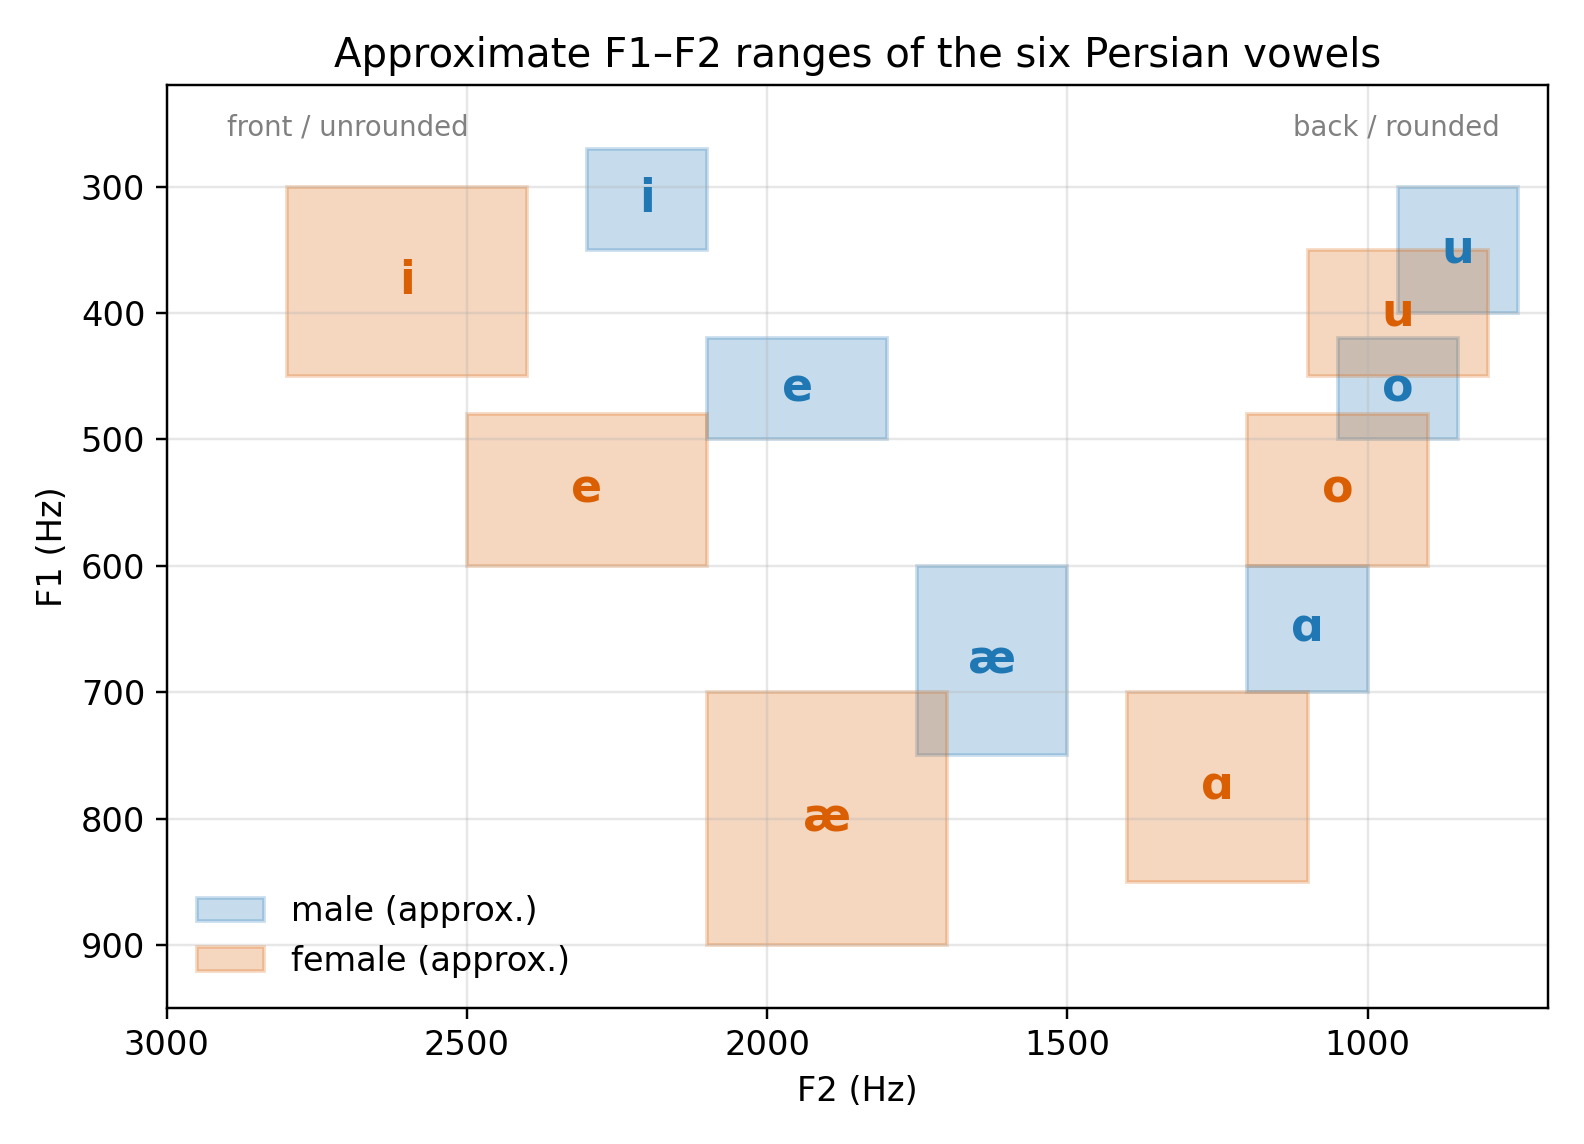
\includegraphics[width=0.85\textwidth]{../assets/figures/ch04-persian-vowel-chart.png}
  \caption{نمودار \eng{F1–F2} برای شش واکهٔ فارسی بر پایهٔ دامنه‌های جدول بالا؛ مستطیل‌ها دامنهٔ تقریبی مردان (آبی) و زنان (نارنجی) را نشان می‌دهند. محورها معکوس‌اند. مقادیر تقریبی‌اند (شکل افزوده).}
\end{figure}

\begin{addedbox}{مقایسه: داده‌های \eng{Peterson \& Barney} برای انگلیسی}
پژوهش کلاسیک \eng{Peterson \& Barney} (۱۹۵۲) فرمنت‌های واکه‌های انگلیسی آمریکایی را برای مردان، زنان و کودکان اندازه گرفت. مقادیر تقریبی \eng{(F1/F2)} برای چهار واکهٔ گوشه (هرتز):
\begin{center}
\begin{tabular}{lccc}
\toprule
واکه & مردان & زنان & کودکان \\
\midrule
\eng{/i/} & ۲۷۰ / ۲۲۹۰ & ۳۱۰ / ۲۷۹۰ & ۳۷۰ / ۳۲۰۰ \\
\eng{/æ/} & ۶۶۰ / ۱۷۲۰ & ۸۶۰ / ۲۰۵۰ & ۱۰۳۰ / ۲۳۲۰ \\
\eng{/ɑ/} & ۷۳۰ / ۱۰۹۰ & ۸۵۰ / ۱۲۲۰ & ۱۰۳۰ / ۱۳۷۰ \\
\eng{/u/} & ۳۰۰ / ۸۷۰ & ۳۷۰ / ۹۵۰ & ۴۳۰ / ۱۱۷۰ \\
\bottomrule
\end{tabular}
\end{center}
هر دو الگوی مهم دیده می‌شود: ترتیب واکه‌ها در همهٔ گروه‌ها یکسان است، ولی مقادیر از مردان به زنان و کودکان بالا می‌روند (به علت کوتاه‌تر شدن مجرای صوتی). پس فضای واکه‌ای هر گروه باید جداگانه ساخته شود. اعداد گردشده و تقریبی‌اند.
\end{addedbox}

\subsection{تفاوت فضای واکه‌ای در گروه‌های مختلف}
فضای واکه‌ای برای همهٔ افراد یکسان نیست. می‌توان آن را جداگانه برای کودکان و بزرگسالان، زنان و مردان، گویندگان زبان‌های مختلف و افراد دارای اختلال یا تفاوت گفتاری استخراج کرد. انتظار داریم رابطهٔ کلی «\eng{F1} با ارتفاع و \eng{F2} با جلوآمدگی» حفظ شود، اما دامنهٔ عددی فرمنت‌ها و پراکندگی واکه‌ها تغییر کند.

\begin{addedbox}{نرمال‌سازی گوینده}
چون اندازهٔ مجرا از گوینده‌ای به گوینده‌ای دیگر فرق می‌کند، برای مقایسهٔ بین گویندگان معمولاً فرمنت‌ها نرمال می‌شوند. یک روش رایج نرمال‌سازی \eng{Lobanov} است: برای هر گوینده و هر فرمنت، مقدار را از میانگین همان گوینده کم و بر انحراف معیار او تقسیم می‌کنند، $z=(F-\mu)/\sigma$. روش‌های دیگر تبدیل به مقیاس‌های ادراکی مانند \eng{Bark} یا \eng{ERB} است. در پایش یک فرد در طول زمان (کاربرد زیستی) نیازی به نرمال‌سازی بین‌فردی نیست، چون هر فرد با خودش مقایسه می‌شود.
\end{addedbox}

\subsection{مساحت فضای واکه‌ای (\eng{VSA})}
برای تبدیل «گستردگی فضای واکه‌ای» به یک عدد، معمولاً مساحت چندضلعی ساخته‌شده از واکه‌های گوشهٔ نمودار \eng{F1–F2} محاسبه می‌شود. تعریف مقالهٔ \eng{Sandoval} و همکاران (۲۰۱۳) که روی تخته آمده این است: \eng{VSA} مساحت دوبعدی محدود به خطوط واصل مختصات \eng{F1/F2} واکه‌های گوشه است؛ در روش سنتی \eng{F1/F2} هر یک از چهار واکهٔ گوشه (یا سه واکهٔ \eng{/a, i, u/} برای مثلث) در ۵۰ درصد مدت واکه چندین بار اندازه گرفته و میانگین‌گیری می‌شود. چون \eng{F1} با باز بودن فک و \eng{F2} با موقعیت زبان مرتبط است، \eng{VSA} نمایندهٔ آکوستیکی جابه‌جایی‌های اندام‌های گفتار است و در گفتار واضح‌تر و قابل‌فهم‌تر بزرگ‌تر است.

\boardfigure{0.45}{ch04-sandoval-vsa-paper.png}{صفحهٔ نخست مقالهٔ \eng{Automatic assessment of vowel space area} (\eng{Sandoval} و همکاران، \eng{JASA Express Letters}، ۲۰۱۳) دربارهٔ تخمین خودکار مساحت فضای واکه‌ای.}

\begin{definitionbox}{محاسبهٔ \eng{VSA} با فرمول شوله‌یس (\eng{Shoelace})}
اگر رأس‌های چندضلعی با ترتیب پیرامونی $(F_{2,k},F_{1,k})$ باشند، مساحت برابر است با
\[
\text{\lr{VSA}}=\frac12\left|\sum_{k=1}^{n}\bigl(F_{2,k}\,F_{1,k+1}-F_{2,k+1}\,F_{1,k}\bigr)\right|,
\]
با قرارداد $k=n+1\equiv 1$. واحد آن $\text{Hz}^2$ است. برای مثلث \eng{(i, a, u)} فرمول بسته چنین است:
\[
\text{\lr{VSA}}_{\triangle}=\frac12\left|F_{1,i}(F_{2,a}-F_{2,u})+F_{1,a}(F_{2,u}-F_{2,i})+F_{1,u}(F_{2,i}-F_{2,a})\right|.
\]
\end{definitionbox}

\begin{addedbox}{مثال عددی: \eng{VSA} مثلثی مردان فارسی‌زبان}
مرکز دامنه‌های جدول مردان را به عنوان مختصات هر واکه می‌گیریم:
\eng{/i/} با $(F_1,F_2)=(310,\,2200)$، \eng{/ɑ/} با $(650,\,1100)$ و \eng{/u/} با $(350,\,850)$ هرتز. بنا بر فرمول بسته:
\begin{align*}
\text{\lr{VSA}}_{\triangle}&=\tfrac12\bigl|310(1100-850)+650(850-2200)+350(2200-1100)\bigr|\\
&=\tfrac12\bigl|77\,500-877\,500+385\,000\bigr|=\tfrac12(415\,000)=207\,500\ \text{Hz}^2.
\end{align*}
اگر \eng{/æ/} با مختصات $(675,1625)$ را هم به‌عنوان چهارمین گوشه اضافه کنیم، چهارضلعی \eng{/i/ $\to$ /æ/ $\to$ /ɑ/ $\to$ /u/} مساحتی برابر $310\,500\ \text{Hz}^2$ دارد.

\textbf{اثر متمرکزشدن.} فرض کنید نقاط هر سه واکه ۲۰ درصد به سمت مرکز ثقل خود (\eng{F1}$=437$، \eng{F2}$=1383$) جمع شوند، یعنی هر فاصله در ضریب $0.8$ ضرب شود. چون مساحت با مربع ضریب مقیاس تغییر می‌کند، مساحت جدید $0.8^2\times207\,500=132\,800\ \text{Hz}^2$ است، یعنی حدود ۳۶ درصد کاهش، هرچند فاصلهٔ هر نقطه فقط ۲۰ درصد کم شده است. بنابراین \eng{VSA} حساس به متمرکز شدن واکه‌ها است.
\end{addedbox}

\begin{figure}[htbp]
  \centering
  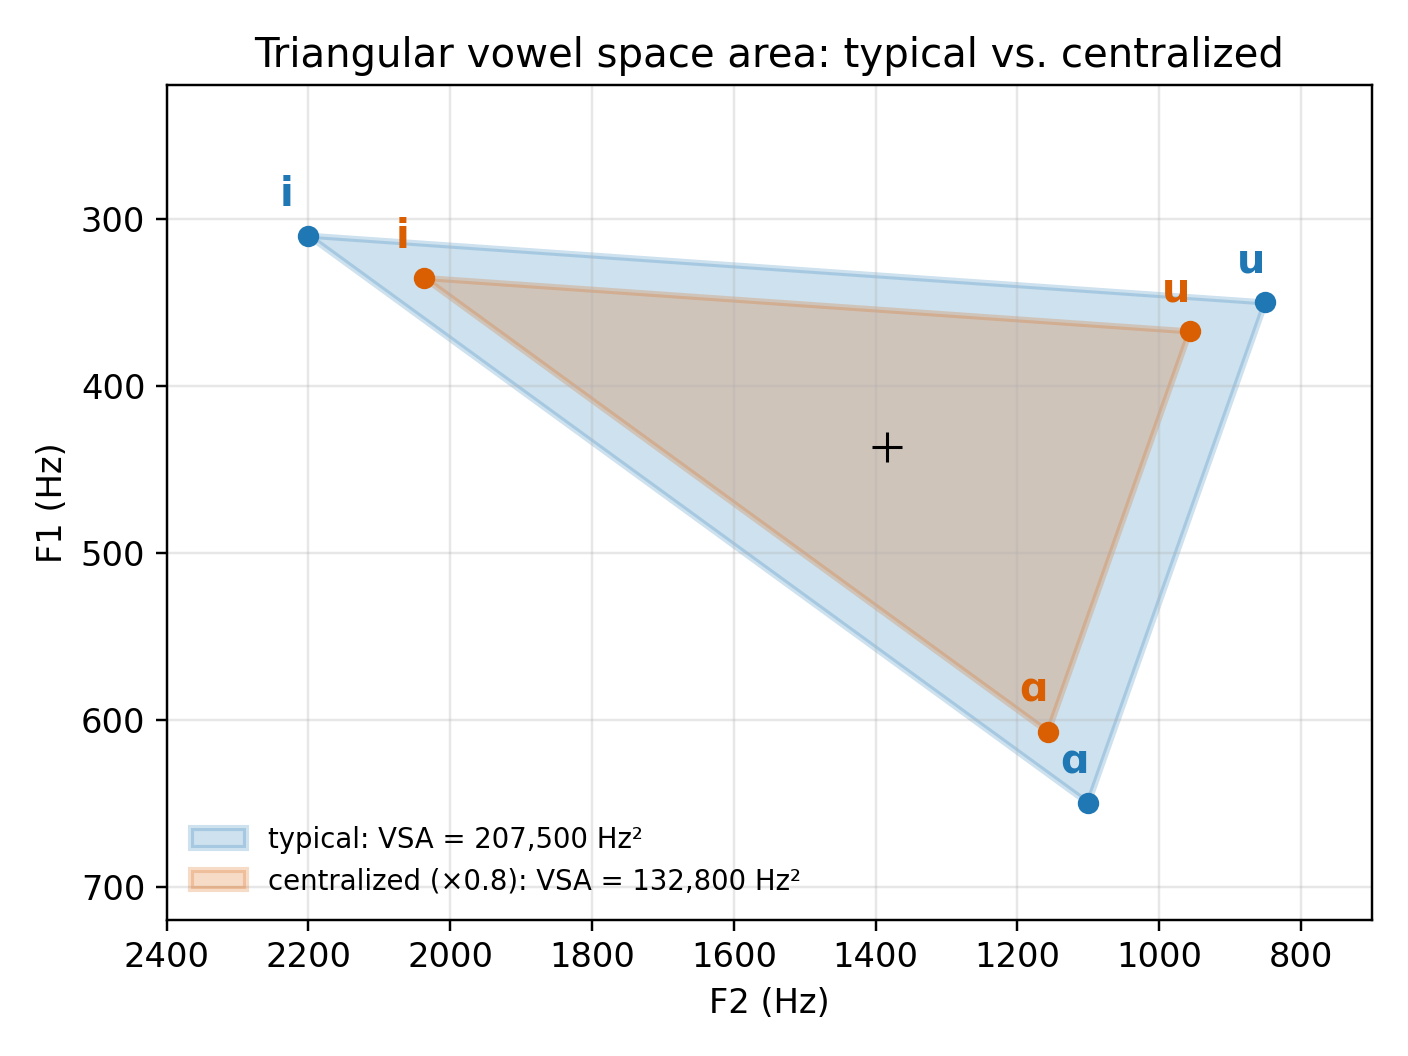
\includegraphics[width=0.75\textwidth]{../assets/figures/ch04-vsa-triangle.png}
  \caption{مثلث \eng{/i, ɑ, u/} برای مقادیر مثال بالا (آبی) و حالت متمرکزشدهٔ آن (نارنجی)؛ کوچک‌شدن مساحت از $207\,500$ به $132\,800$ هرتز مربع. اعداد تقریبی‌اند (شکل افزوده).}
\end{figure}

\begin{addedbox}{شاخص‌های وابسته: \eng{VAI} و \eng{FCR}}
\eng{VSA} به اندازهٔ مجرای گوینده حساس است. برای کاهش این وابستگی \eng{Sapir} و همکاران (۲۰۱۰) نسبت‌هایی را پیشنهاد کردند:
\[
\text{\lr{VAI}}=\frac{F_{2,i}+F_{1,a}}{F_{2,u}+F_{2,a}+F_{1,i}+F_{1,u}},\qquad
\text{\lr{FCR}}=\frac{F_{2,u}+F_{2,a}+F_{1,i}+F_{1,u}}{F_{2,i}+F_{1,a}}=\frac{1}{\text{\lr{VAI}}}.
\]
با متمرکز شدن واکه‌ها \eng{VAI} کاهش و \eng{FCR} افزایش می‌یابد. با مقادیر مثال بالا: \eng{VAI} $=(2200+650)/(850+1100+310+350)\approx1.09$ و پس از متمرکزشدن ($0.8$) حدود $0.94$؛ یا معادلاً \eng{FCR} از $0.92$ به $1.07$ می‌رسد. این شاخص‌ها چون نسبتی‌اند، به مقیاس کلی فرمنت‌ها کمتر وابسته‌اند.
\end{addedbox}

\section{همخوان‌ها در اسپکتروگرام}
یکی از دانشجویان پرسید آیا این تحلیل فقط برای واکه‌هاست. پاسخ استاد: همخوان‌ها هم ویژگی‌های آکوستیکی خاص خود را دارند و در اسپکتروگرام قابل بررسی‌اند، ولی تمرکز فعلی درس روی واکه‌ها و فضای واکه‌ای است و همخوان‌ها موضوع مطالعهٔ بیشتر است.

\begin{assignmentbox}{تمرین پیشنهادی استاد}
بررسی کنید همخوان‌ها (\eng{Consonants}) چگونه در اسپکتروگرام دیده می‌شوند و آیا اسپکتروگرام با آنچه در آواشناسی تولیدی گفتیم هماهنگ است. روی تخته نوشته شده: «بله، با \textbf{سکوت} (شیوهٔ تولید) و نحوهٔ \textbf{خم‌شدن و جهش فرمنت‌ها} و \textbf{مرکز فرکانسی نویز} (جایگاه تولید)، حرکات فیزیکی اندام‌های گفتاری را کدگذاری می‌کند.» به‌خصوص این موارد را بررسی کنید:
\begin{itemize}
  \item سکوت یا انسداد پیش از برخی همخوان‌ها؛
  \item انفجار (\eng{Burst}) در همخوان‌های انسدادی مانند \eng{/b/} و \eng{/p/};
  \item تغییر شکل فرمنت‌ها هنگام گذار از همخوان به واکه (\eng{Formant Transitions});
  \item تفاوت الگوهای زمانی و فرکانسی همخوان‌ها.
\end{itemize}
\end{assignmentbox}

\begin{addedbox}{راهنمای خوانش همخوان‌ها در طیف‌نگاره}
\begin{itemize}
  \item \textbf{شیوهٔ تولید:} همخوان‌های انسدادی ($/p,t,k,b,d,g/$) یک بازهٔ بسته با انرژی بسیار کم دارند (در واک‌دارها یک نوار فرکانس پایین به نام \eng{voice bar})، سپس یک انفجار کوتاه و زمان آغاز واک (\eng{VOT}). سایشی‌ها ($/s,\,\text{\lr{ʃ}},f/$) نویز پیوسته با انرژی پهن‌باند دارند. خیشومی‌ها فرمنت‌های ضعیف و یک ناحیهٔ ضدتشدید دارند.
  \item \textbf{جایگاه تولید:} در سایشی‌ها مرکز ثقل نویز مهم است: \eng{/s/} انرژی را در فرکانس‌های بالا (حدود بالای ۴۰۰۰ هرتز) و \eng{/ʃ/} در فرکانس‌های پایین‌تر (حدود ۲۰۰۰ تا ۳۰۰۰ هرتز) دارد. در انسدادی‌ها جهت گذار \eng{F2} و \eng{F3} به واکهٔ بعد (مثلاً بالارفتن \eng{F2} پس از همخوان دولبی) نشان‌دهندهٔ جایگاه تولید است.
\end{itemize}
\end{addedbox}

\section{کاربردهای فضای واکه‌ای}
پس از ساخت فضای واکه‌ای گوینده یا گروه، استاد از دانشجویان پرسید چه کاربردی دارد. پاسخ‌های اولیه (تشخیص واکه، آموزش مدل و پیش‌پردازش) کافی نبود: فضای واکه‌ای قبل از هر چیز ابزار \emph{تحلیل ساختار تولید گفتار}، مقایسهٔ گروه‌ها و شناسایی الگوهای متفاوت است. روی تخته سه کاربرد اصلی نوشته شده بود.

\subsection{گفتاردرمانی و بازخورد زیستی تصویری}
\term{بیوفیدبک تصویری}{Visual Biofeedback}: برای کودکان دارای اختلال گفتاری، ناشنوایان یا افراد مبتلا به سندرم داون، نمایشگری زنده نشان داده می‌شود که با حرکت دادن زبان، یک نقطه روی نمودار (\eng{F1} و \eng{F2}) حرکت می‌کند. کودک یاد می‌گیرد چگونه زبانش را بالا ببرد تا نقطه به هدف مشخص‌شده روی نقشه برسد. ایده این است که فضای واکهٔ مرجع را داشته باشیم، گفتار فرد را اندازه بگیریم و اختلاف را نشان دهیم؛ مثلاً اگر واکه‌ای با \eng{F1} بالاتر از هدف تولید شود، بازخوردی دربارهٔ تغییر ارتفاع زبان داده شود. مزیت: بازخورد از حالت صرفاً شنیداری و کلامی به شکل دیداری درمی‌آید.

\begin{warningbox}{محدودیت‌های عملی}
چنین بازخوردی را باید با توجه به ویژگی‌های واکه و شرایط فرد تفسیر کرد. در گفتار کودکان و زنان که $f_0$ بالا است و هارمونیک‌ها از هم دور هستند، تخمین فرمنت دشوار و ناپایدار است و نقطهٔ نمایش‌داده‌شده ممکن است بپرد. بهتر است هدف را یک \emph{ناحیه} (بیضی دامنهٔ واکه) در نظر بگیریم، نه نقطه، و فرمنت‌ها را هموار کنیم.
\end{warningbox}

\subsection{تشخیص صدای جعلی (\eng{Deepfake})}
مدل‌های تولید گفتار می‌توانند صدایی بسازند که برای گوش انسان طبیعی است، اما طبیعی‌بودن شنیداری به معنای یکسان‌بودن همهٔ ویژگی‌های آکوستیکی و تولیدی با گفتار واقعی نیست. ایده: فرمنت‌های واکه‌ها را برای نمونهٔ واقعی و نمونهٔ سنتز‌شده استخراج و فضای واکه‌ای آن‌ها را مقایسه کنیم؛ اگر تفاوت معنادار و قابل‌اتکایی وجود داشته باشد، می‌توان از آن‌ها به‌عنوان ویژگی تشخیص جعل استفاده کرد. به گفتهٔ روی تخته: گفتار سنتز‌شده در مقایسه با گفتار واقعی ناهماهنگی‌هایی در هندسه و تغییر شکل مجرای صوتی نشان می‌دهد؛ و «تفاوت‌های بیومکانیکی در تلفظ مصوت‌ها بهترین ردپای مصنوعی‌بودن صدا هستند». استاد همچنین به هم‌بستگی (\eng{Correlation}) میان ویژگی‌های آکوستیکی گفتار واقعی و تولیدی اشاره کرد: می‌توان بررسی کرد آیا الگوی تغییر \eng{F1} و \eng{F2} در واکه‌های مختلف با گفتار طبیعی سازگار است. روی تخته نام «\eng{Siwei Lyu}» (پژوهشگر شناخته‌شدهٔ حوزهٔ تشخیص دیپ‌فیک) نیز در همین بخش آمده است.

استاد مقاله‌ای را نشان داد که از ویژگی‌های مرتبط با تولید و شکل مجرای صوتی برای تشخیص گفتار مصنوعی استفاده می‌کند.

\begin{figure}[htbp]
  \centering
  \begin{minipage}{0.45\textwidth}
    \centering
    \fbox{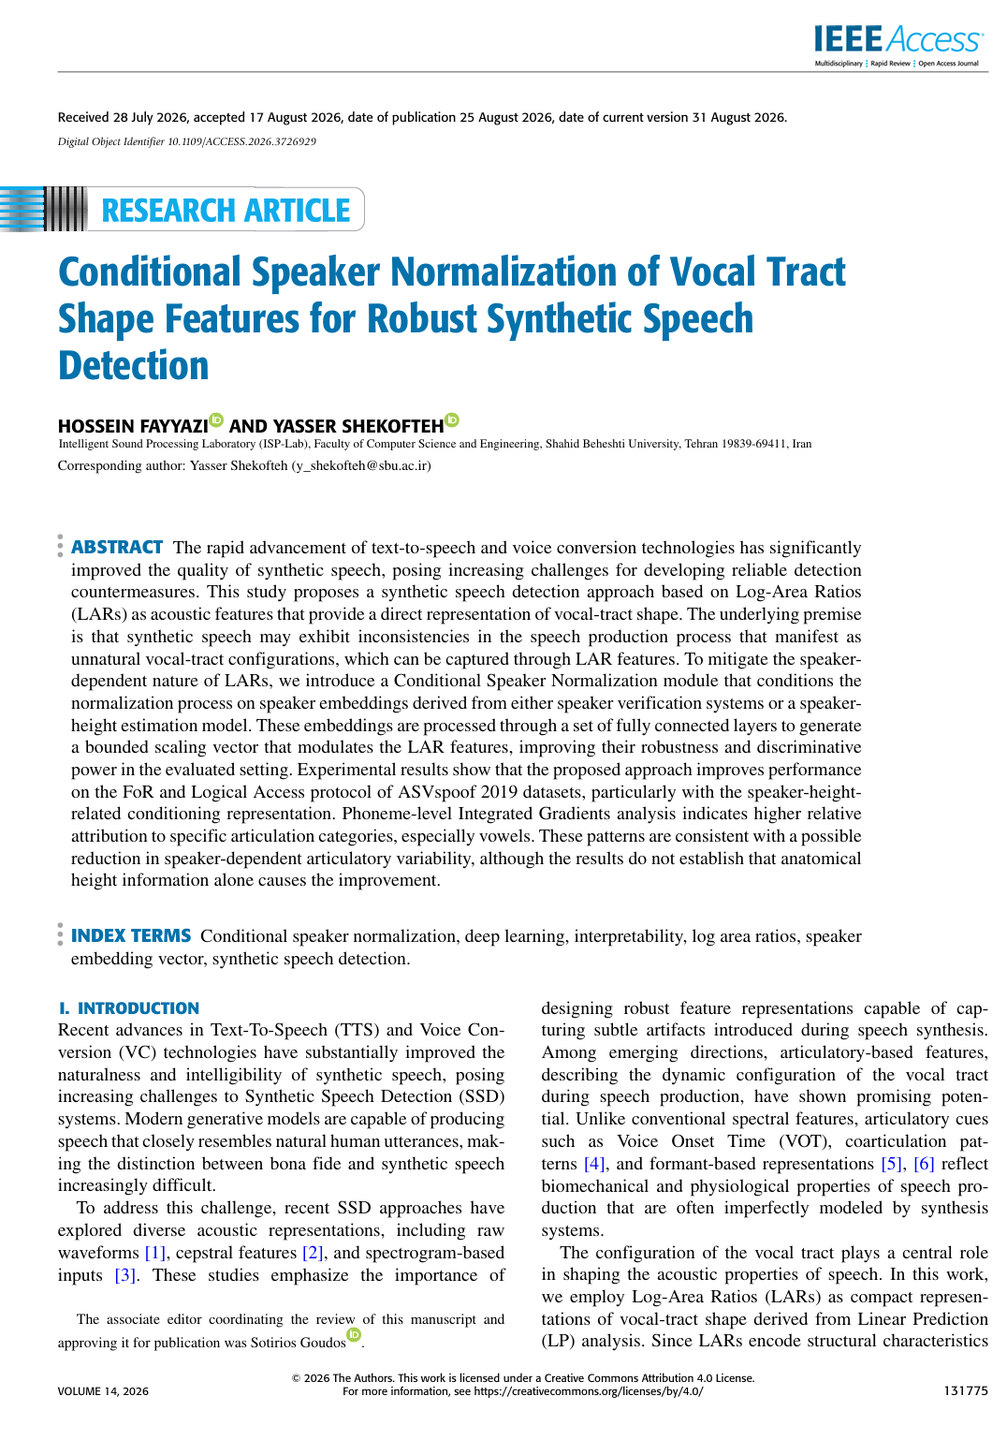
\includegraphics[width=\textwidth]{../assets/figures/ch04-fayyazi-paper.png}}
    \caption*{مقالهٔ \eng{Conditional Speaker Normalization of Vocal Tract Shape Features for Robust Synthetic Speech Detection} (\eng{IEEE Access}، ۲۰۲۶).}
  \end{minipage}\hfill
  \begin{minipage}{0.5\textwidth}
    \centering
    \fbox{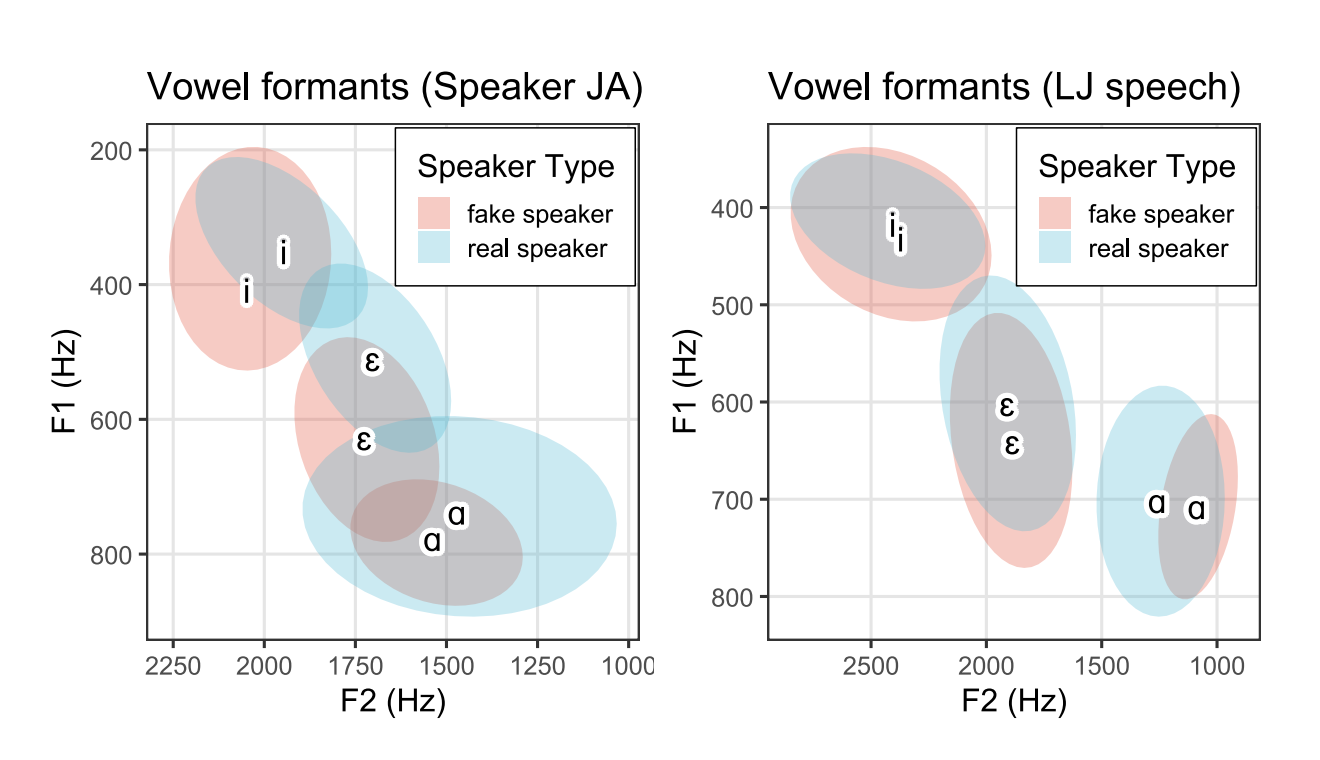
\includegraphics[width=\textwidth]{../assets/figures/ch04-fake-real-vowels.png}}
    \caption*{بیضی‌های \eng{F1–F2} برای چند واکه در صدای واقعی (آبی) و جعلی (قرمز) برای دو گوینده/پیکره.}
  \end{minipage}
  \caption{نمونهٔ استفاده از فضای واکه‌ای و شکل مجرا برای تشخیص گفتار جعلی \textit{(برگرفته از تختهٔ کلاس)}}
\end{figure}

\begin{correctionbox}{«اثبات» جعل؟}
عبارت روی تخته دربارهٔ «اثبات جعل در محیط‌های جرم‌شناسی» باید با احتیاط خوانده شود. روش‌های مبتنی بر فضای واکه‌ای یا شکل مجرا شواهد آماری تولید می‌کنند، نه اثبات قطعی. نمودار روی تخته هم نشان می‌دهد در بسیاری از واکه‌ها بیضی‌های واقعی و جعلی هم‌پوشانی زیادی دارند و فقط در برخی واکه‌ها یا گویندگان جابه‌جایی دیده می‌شود. خود مقالهٔ نشان‌داده‌شده (چکیدهٔ آن) می‌گوید بهبود حاصل با الگوهای سازگار با کاهش تغییرپذیری تولیدی وابسته به گوینده هم‌خوان است، اما نتایج نشان نمی‌دهد که صرف اطلاعات قد گوینده علت بهبود باشد. استاد هم تأکید کرد گزارهٔ کلی «فرمنت‌ها فرق دارند» برای پژوهش علمی کافی نیست؛ باید معلوم شود:
\begin{enumerate}
  \item دقیقاً کدام ویژگی آکوستیکی تفاوت دارد؟
  \item چگونه اندازه‌گیری می‌شود؟
  \item آیا در نمونه‌های مختلف تکرارپذیر است؟
  \item آیا می‌توان با آن گفتار واقعی و مصنوعی را قابل‌اعتماد تفکیک کرد؟
\end{enumerate}
\end{correctionbox}

\subsubsection{مقاوم‌سازی مدل (\eng{Robustness})}
استاد پرسید اگر نقاط ضعف یک مدل را شناسایی کردیم، چگونه آن را مقاوم‌تر کنیم؟ پاسخ: استفادهٔ هدفمند از داده‌هایی که مدل در آن‌ها ضعف دارد؛ مثلاً اگر مدل در برخی واکه‌ها ضعیف‌تر است، از همان واکه‌ها دادهٔ بیشتر جمع و به مجموعهٔ آموزش اضافه شود. روش‌های مرتبط: \eng{Data Augmentation} (افزایش و متنوع‌سازی دادهٔ آموزشی)، \eng{Hard Example Mining} (تمرکز بر نمونه‌های دشوار) و \eng{Adversarial Training}. پیش‌شرط این کار دانستن این است که مدل \emph{دقیقاً کجا} ضعف دارد، و تحلیل فضای واکه‌ای می‌تواند یکی از راه‌های شناسایی چنین نقاطی باشد.

\subsection{نشانگر زیستی دیجیتال (\eng{Digital Biomarker})}
\begin{definitionbox}{نشانگر زیستی دیجیتال}
ویژگی قابل‌اندازه‌گیری‌ای که با ابزارهای دیجیتال به دست می‌آید و دربارهٔ وضعیت یا تغییرات یک فرایند زیستی یا بالینی اطلاعات می‌دهد. ویژگی‌های آکوستیکی گفتار می‌توانند تغییر توانایی تولید گفتار را در طول زمان نشان دهند.
\end{definitionbox}

روی تخته: «شاخص بیومارکر دیجیتال برای تعیین پیشرفت بیماری‌های نورولوژیک درگیرکنندهٔ کنترل حرکتی گفتار مثل دمانس یا پارکینسون». در این بیماری‌ها مقادیر فرمنت اول و دوم به سمت مرکز فضای صوتی جمع می‌شوند (\term{متمرکزشدن}{Centralization}) و مساحت فضای واکه‌ای کوچک می‌شود. وقتی فرد بتواند واکه‌ها را متمایز تولید کند، نقاط واکه‌های مختلف در فضای \eng{F1–F2} از هم فاصله دارند؛ با دشوارشدن تمایزهای تولیدی، واکه‌ها به ناحیهٔ مرکزی نزدیک می‌شوند. اندازه‌گیری مکرر در طول زمان می‌تواند تغییراتی را نشان دهد که شنوندهٔ عادی هنوز نمی‌شنود.

\begin{figure}[htbp]
\centering
\begin{tikzpicture}[rtl, scale=1.0]
  \begin{scope}[xshift=6cm]
    \draw[fill=blue!15, draw=blue!60!black, thick] (0,0) -- (3,0.2) -- (2.3,2.5) -- cycle;
    \node[font=\small] at (1.8,-0.55) {فضای گسترده};
    \node[font=\small] at (1.8,-1.05) {تمایز بیشتر واکه‌ها};
    \node[font=\scriptsize] at (-0.2,-0.2) {\lr{/i/}};
    \node[font=\scriptsize] at (3.3,0.2) {\lr{/u/}};
    \node[font=\scriptsize] at (2.3,2.8) {\lr{/a/}};
  \end{scope}
  \begin{scope}
    \draw[fill=orange!20, draw=orange!70!black, thick] (0.8,0.65) -- (2.2,0.75) -- (1.9,1.7) -- cycle;
    \node[font=\small] at (1.5,-0.55) {فضای متمرکز};
    \node[font=\small] at (1.5,-1.05) {کاهش فاصلهٔ واکه‌ها};
    \node[font=\scriptsize] at (0.5,0.55) {\lr{/i/}};
    \node[font=\scriptsize] at (2.5,0.75) {\lr{/u/}};
    \node[font=\scriptsize] at (1.9,2.0) {\lr{/a/}};
  \end{scope}
  \draw[-{Stealth}, thick] (5.2,1.0) -- (3.9,1.0);
\end{tikzpicture}
\caption{نمایش شماتیک متمرکزشدن فضای واکه‌ای: مثلث واکه‌ها کوچک می‌شود و به مرکز نزدیک می‌شود (شکل افزوده).}
\end{figure}

\subsubsection{پایش تغییرات گفتار برای تشخیص زودهنگام}
هدف نوشته‌شده روی تخته «تخمین تمام خودکار فضای واکه‌ای» و «اندازه‌گیری کمّی و تشخیص زودهنگام» بود. مقالهٔ \eng{Sandoval} و همکاران (۲۰۱۳) الگوریتمی خودکار برای تخمین \eng{VSA} از گفتار پیوستهٔ سالم، به‌جای هجاهای جدا، ارائه می‌کند که کل «فضای کاری» واکه‌ها را در نظر می‌گیرد و همبستگی بالایی با \eng{VSA} سنتی دارد؛ در موارد اختلاف، روش خودکار دقیق‌تر ارزیابی شده چون همهٔ واکه‌ها را به حساب می‌آورد. روند پایش پیشنهادی:
\begin{enumerate}
  \item از فرد خواسته می‌شود هر چند وقت یک بار مجموعه‌ای از واکه‌ها یا جملات مشخص را ضبط کند.
  \item فرمنت‌ها استخراج می‌شوند.
  \item فضای واکه‌ای ساخته می‌شود.
  \item گستردگی و پراکندگی واکه‌ها اندازه‌گیری می‌شود.
  \item با نمونه‌های قبلی همان فرد مقایسه می‌شود.
  \item در صورت تغییر قابل‌توجه، بررسی تخصصی پیشنهاد می‌شود.
\end{enumerate}
استاد ایدهٔ ساخت سامانه‌ای را مطرح کرد که از طریق \textbf{تلفن همراه} نمونه‌های گفتار را در طول زمان دریافت و تحلیل کند و تغییرات احتمالی را اعلام کند.

\begin{correctionbox}{نشانگر زیستی دیجیتال ابزار تشخیص قطعی نیست}
شواهد پژوهشی کاهش \eng{VSA} یا \eng{VAI} در برخی افراد مبتلا به بیماری پارکینسون و سایر دیزآرتری‌های حرکتی را نشان می‌دهند (از جمله مطالعهٔ \eng{Sapir} و همکاران ۲۰۱۰ دربارهٔ \eng{FCR}). اما اثر آن در همهٔ بیماران، همهٔ مراحل و همهٔ واکه‌ها یکسان نیست، و برای دمانس شواهد غیرمستقیم‌تر و ضعیف‌تر است. عبارت «مساحت به شدت کوچک می‌شود» روی تخته را باید حالت شدید بیماری دانست، نه قاعدهٔ عمومی. این شاخص‌ها به‌تنهایی ابزار قطعی تشخیص پارکینسون یا دمانس نیستند و کاربرد بالینی آن‌ها به اعتبارسنجی بالینی و تفسیر متخصص نیاز دارد. همچنین عواملی مانند سن، جنس، خستگی، کیفیت میکروفون تلفن و نویز محیط می‌توانند \eng{VSA} را تغییر دهند و باید کنترل شوند. متن پیاده‌شدهٔ جلسه در همین بحث، پیش از تکمیل جملهٔ پایانی استاد، قطع می‌شود.
\end{correctionbox}

\section{جمع‌بندی}
هدف این جلسه فقط استخراج فرکانس از سیگنال نبود: با اندازه‌گیری \eng{F1} و \eng{F2} در \eng{Praat} می‌توان بازنمایی‌ای از الگوی تولید واکه‌ها ساخت. \eng{F1} با ارتفاع زبان رابطهٔ معکوس و \eng{F2} با جلو یا عقب بودن زبان (و گردی لب) رابطه دارد. با برچسب‌گذاری \eng{TextGrid} و بازهٔ هر واکه، جدول فرمنت‌ها برای هر گروه ساخته می‌شود و در نمودار \eng{F1–F2} با محورهای معکوس فضای واکه‌ای شکل می‌گیرد. برای ساخت پیکرهٔ جامعهٔ خاص (مثلاً کودکان) می‌توان از \eng{ASR} برای متن اولیه و از بازبینی انسانی برای اصلاح بهره برد. مساحت فضای واکه‌ای و شاخص‌هایی مانند \eng{VAI} مقدار عددی گستردگی فضا را می‌دهند. این بازنمایی امکان مقایسهٔ گویندگان و گروه‌ها، گفتاردرمانی تصویری، تشخیص صدای مصنوعی و پایش تغییرات گفتار (نشانگر زیستی دیجیتال) را فراهم می‌کند؛ اما همهٔ این کاربردها نیاز به اعتبارسنجی دقیق و تفسیر محتاطانه دارند.

\begin{exambox}{نکات مهم برای مرور و امتحان}
\begin{center}
\small
\begin{tabular}{p{3.6cm}p{10cm}}
\toprule
مفهوم & نکتهٔ اصلی \\
\midrule
فرکانس پایه & فرکانس تکرار دورهٔ اصلی سیگنال تناوبی؛ $f_0=1/T$؛ مربوط به منبع \\
\eng{Magnitude} & اندازهٔ ضریب فوریه و نه دامنهٔ زمانی سیگنال \\
تعامد & صفرشدن ضرب داخلی دو سیگنال؛ لازم برای موج‌های مبنا \\
هارمونیک‌ها & مضرب‌های صحیح $f_0$؛ در موج مربعی فقط مضرب‌های فرد \\
فرمنت‌ها & ناحیه‌های تشدید مجرا (فیلتر)؛ تخمین با \eng{LPC} \\
\eng{Wideband} / \eng{Narrowband} & تفکیک زمانی (فرمنت) در برابر تفکیک فرکانسی (هارمونیک) \\
\eng{F1} & رابطهٔ معکوس با ارتفاع زبان \\
\eng{F2} & رابطهٔ مستقیم با جلو آمدن زبان؛ گردشدن لب‌ها \eng{F2} را کاهش می‌دهد \\
\eng{Praat} & ضبط، تحلیل (\eng{Pitch}، \eng{Formant}، \eng{Spectrogram}، \eng{Intensity})، برچسب‌گذاری \\
\eng{TextGrid} & لایه‌های \eng{Word}، \eng{Syllable}، \eng{Phoneme} \\
فضای واکه‌ای & نمودار \eng{F1–F2} با هر دو محور معکوس؛ برای هر گروه جداگانه \\
\eng{ASR} + بازبینی انسانی & ساخت سریع‌تر پیکره؛ مستندسازی برچسب‌گذاری ضروری \\
\eng{VSA} & مساحت چندضلعی واکه‌های گوشه در \eng{F1–F2}؛ کوچک‌شدن = متمرکزشدن \\
کاربردها & گفتاردرمانی (بیوفیدبک تصویری)، تشخیص جعل، نشانگر زیستی دیجیتال \\
\bottomrule
\end{tabular}
\end{center}
\textbf{زنجیرهٔ جلسه:} سیگنال صوتی $\leftarrow$ استخراج ویژگی‌های آکوستیکی (\eng{Pitch}، طیف، فرمنت) $\leftarrow$ اندازه‌گیری \eng{F1}/\eng{F2} در \eng{Praat} $\leftarrow$ ساخت فضای واکه‌ای $\leftarrow$ مقایسه با الگوی مرجع یا گروه‌های دیگر $\leftarrow$ کاربردهای پژوهشی و عملی.
\end{exambox}
